% ----------------------------------------------	
\pagestyle{plain}
\whitetext{\chapter{Introduction}}
\pagecolor{ccteal}
\fontfamily{phv}
%\vspace*{\stretch{.5}}
\pagebreak
\newpagecolor{white}
\pagestyle{fancy}
\fancyhf{}
\renewcommand{\chaptermark}[1]{\markboth{#1}{}}
\fancyfoot[LE,RO]{\thepage}

	\begin{minipage}[t][.5\textheight][t]{\textwidth}
	\textcolor{ccteal}{\section{Overview}}
	Located in the Bedford-Stuyvesant area of Brooklyn, the Sumner Consolidation is composed of three developments: Sumner Houses, 303 Vernon Avenue, and Bedford-Stuyvesant Rehab. All developments in the consolidation 	receive federal funding. The staff are deployed from the management office located in a Sumner building. Built in 1958, Sumner is a 22-acre development with 13 buildings ranging from
	7-12 floors, which house 1,088 families. The development also features a basketball court, green areas
	and parking lots. Sumner's modern ``towers-in-the-park'' model comes with a trash chute system that is
	designed to streamline household trash collection. While this system is made to be convenient for
	residents, it prioritizes trash over recycling by only having a single small chute. a feature, along with
	larger apartments and large spaces between buildings, was designed to rid urban areas of longtime
	problems concerning health and welfare.
	Like Sumner, 303 Vernon is a conventional development with green spaces and a parking lot. It is a
	24-story building built several years later in the summer of 1967. While it is a standalone building, 303
	Vernon also has a chute system for convenient trash disposal.
	Bedford-Stuyvesant Rehab is a turnkey development acquired by NYCHA in 1983 comprised of five
	buildings between 4-6 stories that were not constructed originally for public housing. These pre-war
	tenement buildings, built in the early 1930s, do not come with a chute system like the other
	developments in Sumner Consolidation. Residents leave their waste at the curb for pickup by NYCHA
	caretakers. This can promote more recycling; however, it is more labor intensive for residents.
	
	\end{minipage}
\begin{minipage}[b][.49\textheight][b]{\textwidth}
\begin{table}[H]
\small

\begin{tabular}{l|c|c|c|c|}
\cline{2-5}
																	   & \cellcolor{ccteal}{\color[HTML]{FFFFFF} TDS \#} & \cellcolor{ccteal}{\color[HTML]{FFFFFF} Total Households} & \cellcolor{ccteal}{\color[HTML]{FFFFFF} Official Population} & \cellcolor{ccteal}{\color[HTML]{FFFFFF} Average Family Size} \\ \hline

\multicolumn{1}{|l|}{\cellcolor{ccteallight}303 Vernon Avenue}        & 156                                                   & 233                                                           & 538                                                                & 2.3                                                                \\ \hline\multicolumn{1}{|l|}{\cellcolor{ccteallight}Bedford-Stuyvesant Rehab}        & 311                                                   & 82                                                           & 193                                                                & 2.4                                                                \\ \hline\multicolumn{1}{|l|}{\cellcolor{ccteallight}Sumner}        & 073                                                   & 1,084                                                           & 2,262                                                                & 2.1                                                                \\ \hline
\end{tabular}
\begin{comment}
\begin{tabular}{l|l|l|l|l|}
\cline{2-5}
																	   & \cellcolor{ccteal}{\color[HTML]{FFFFFF} TDS \#} & \cellcolor{ccteal}{\color[HTML]{FFFFFF} Total Families} & \cellcolor{ccteal}{\color[HTML]{FFFFFF} Official Population} & \cellcolor{ccteal}{\color[HTML]{FFFFFF} Average Family Size} \\ \hline
\multicolumn{1}{|l|}{\cellcolor{ccteallight}303 Vernon Avenue}        & 156                                                   & 233                                                           & 538                                                                & 2.3                                                                \\ \hline
\multicolumn{1}{|l|}{\cellcolor{ccteallight}Bedford-Stuyvesant Rehab} & 311                                                   & 82                                                            & 193                                                                & 2.4                                                                \\ \hline
\multicolumn{1}{|l|}{\cellcolor{ccteallight}Sumner Houses}            & 073                                                   & 1,804                                                         & 2,262                                                              & 2.1                                                                \\ \hline
\end{comment}

\end{table}

\begin{centering}
\begin{table}[H]
\begin{tabular}{m{1.25in} m{2in} m{.1in} m{1.25in} m{2in}}
\sf\bf{Sumner Houses and 303 Vernon Avenue} & 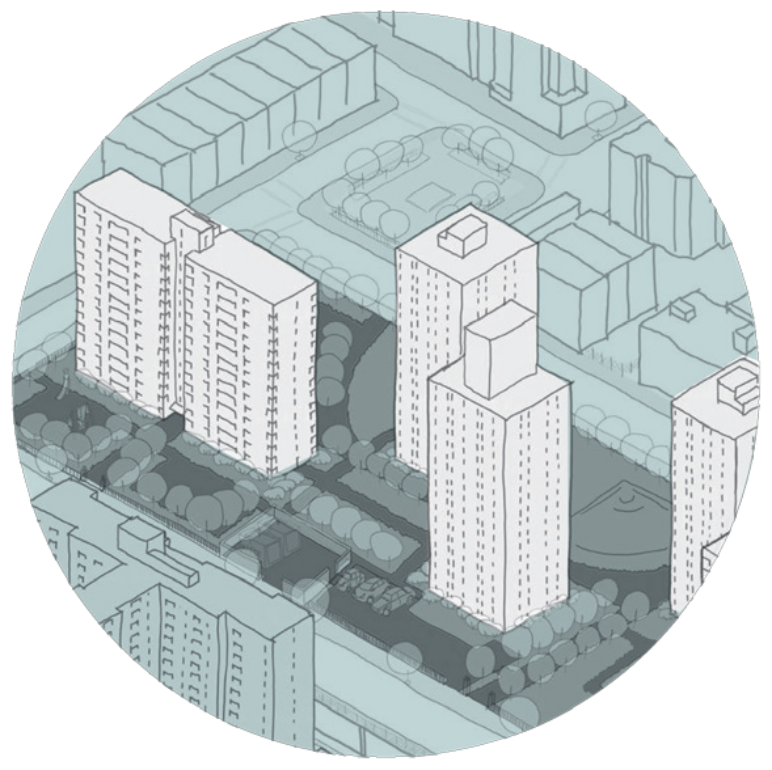
\includegraphics[height=2in]{towers_in_park} & & \sf\bf{Bedford-Stuyvesant Rehab} & 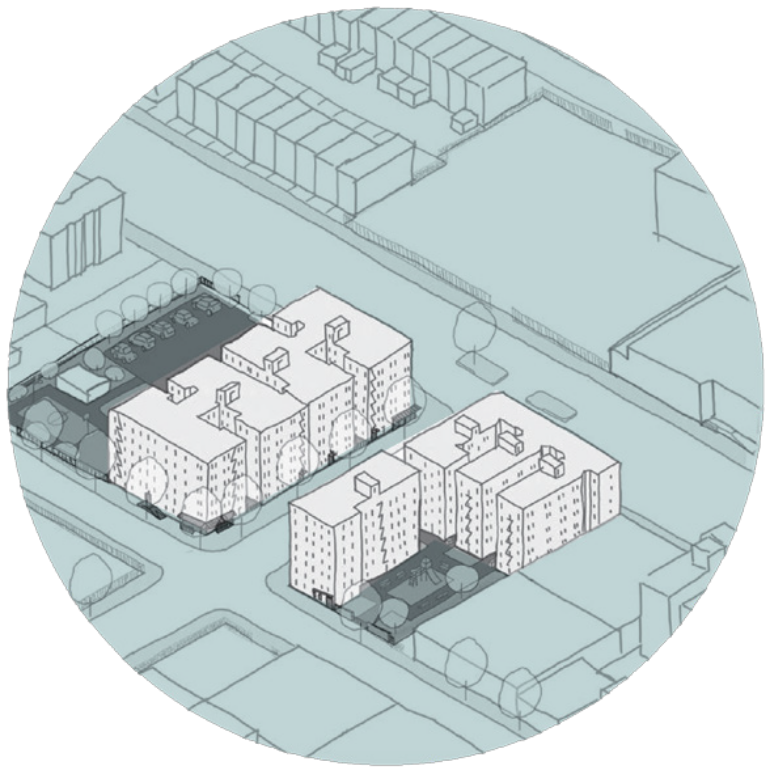
\includegraphics[height=2in]{prewar.png}
\end{tabular}
\end{table}
\end{centering}
\end{minipage}
\pagebreak

\newgeometry{left=0in, right=0in, top=0in, bottom=0in}
\fakesection{Context Map}
\afterpage{%
    \clearpage% flush all other floats
    \ifodd\value{page}
    %\else% uncomment this else to get odd/even instead of even/odd
        \expandafter\afterpage% put it on the next page if this one is odd
    \fi
    {%
    \begin{figure}[H]
    	\raggedleft
        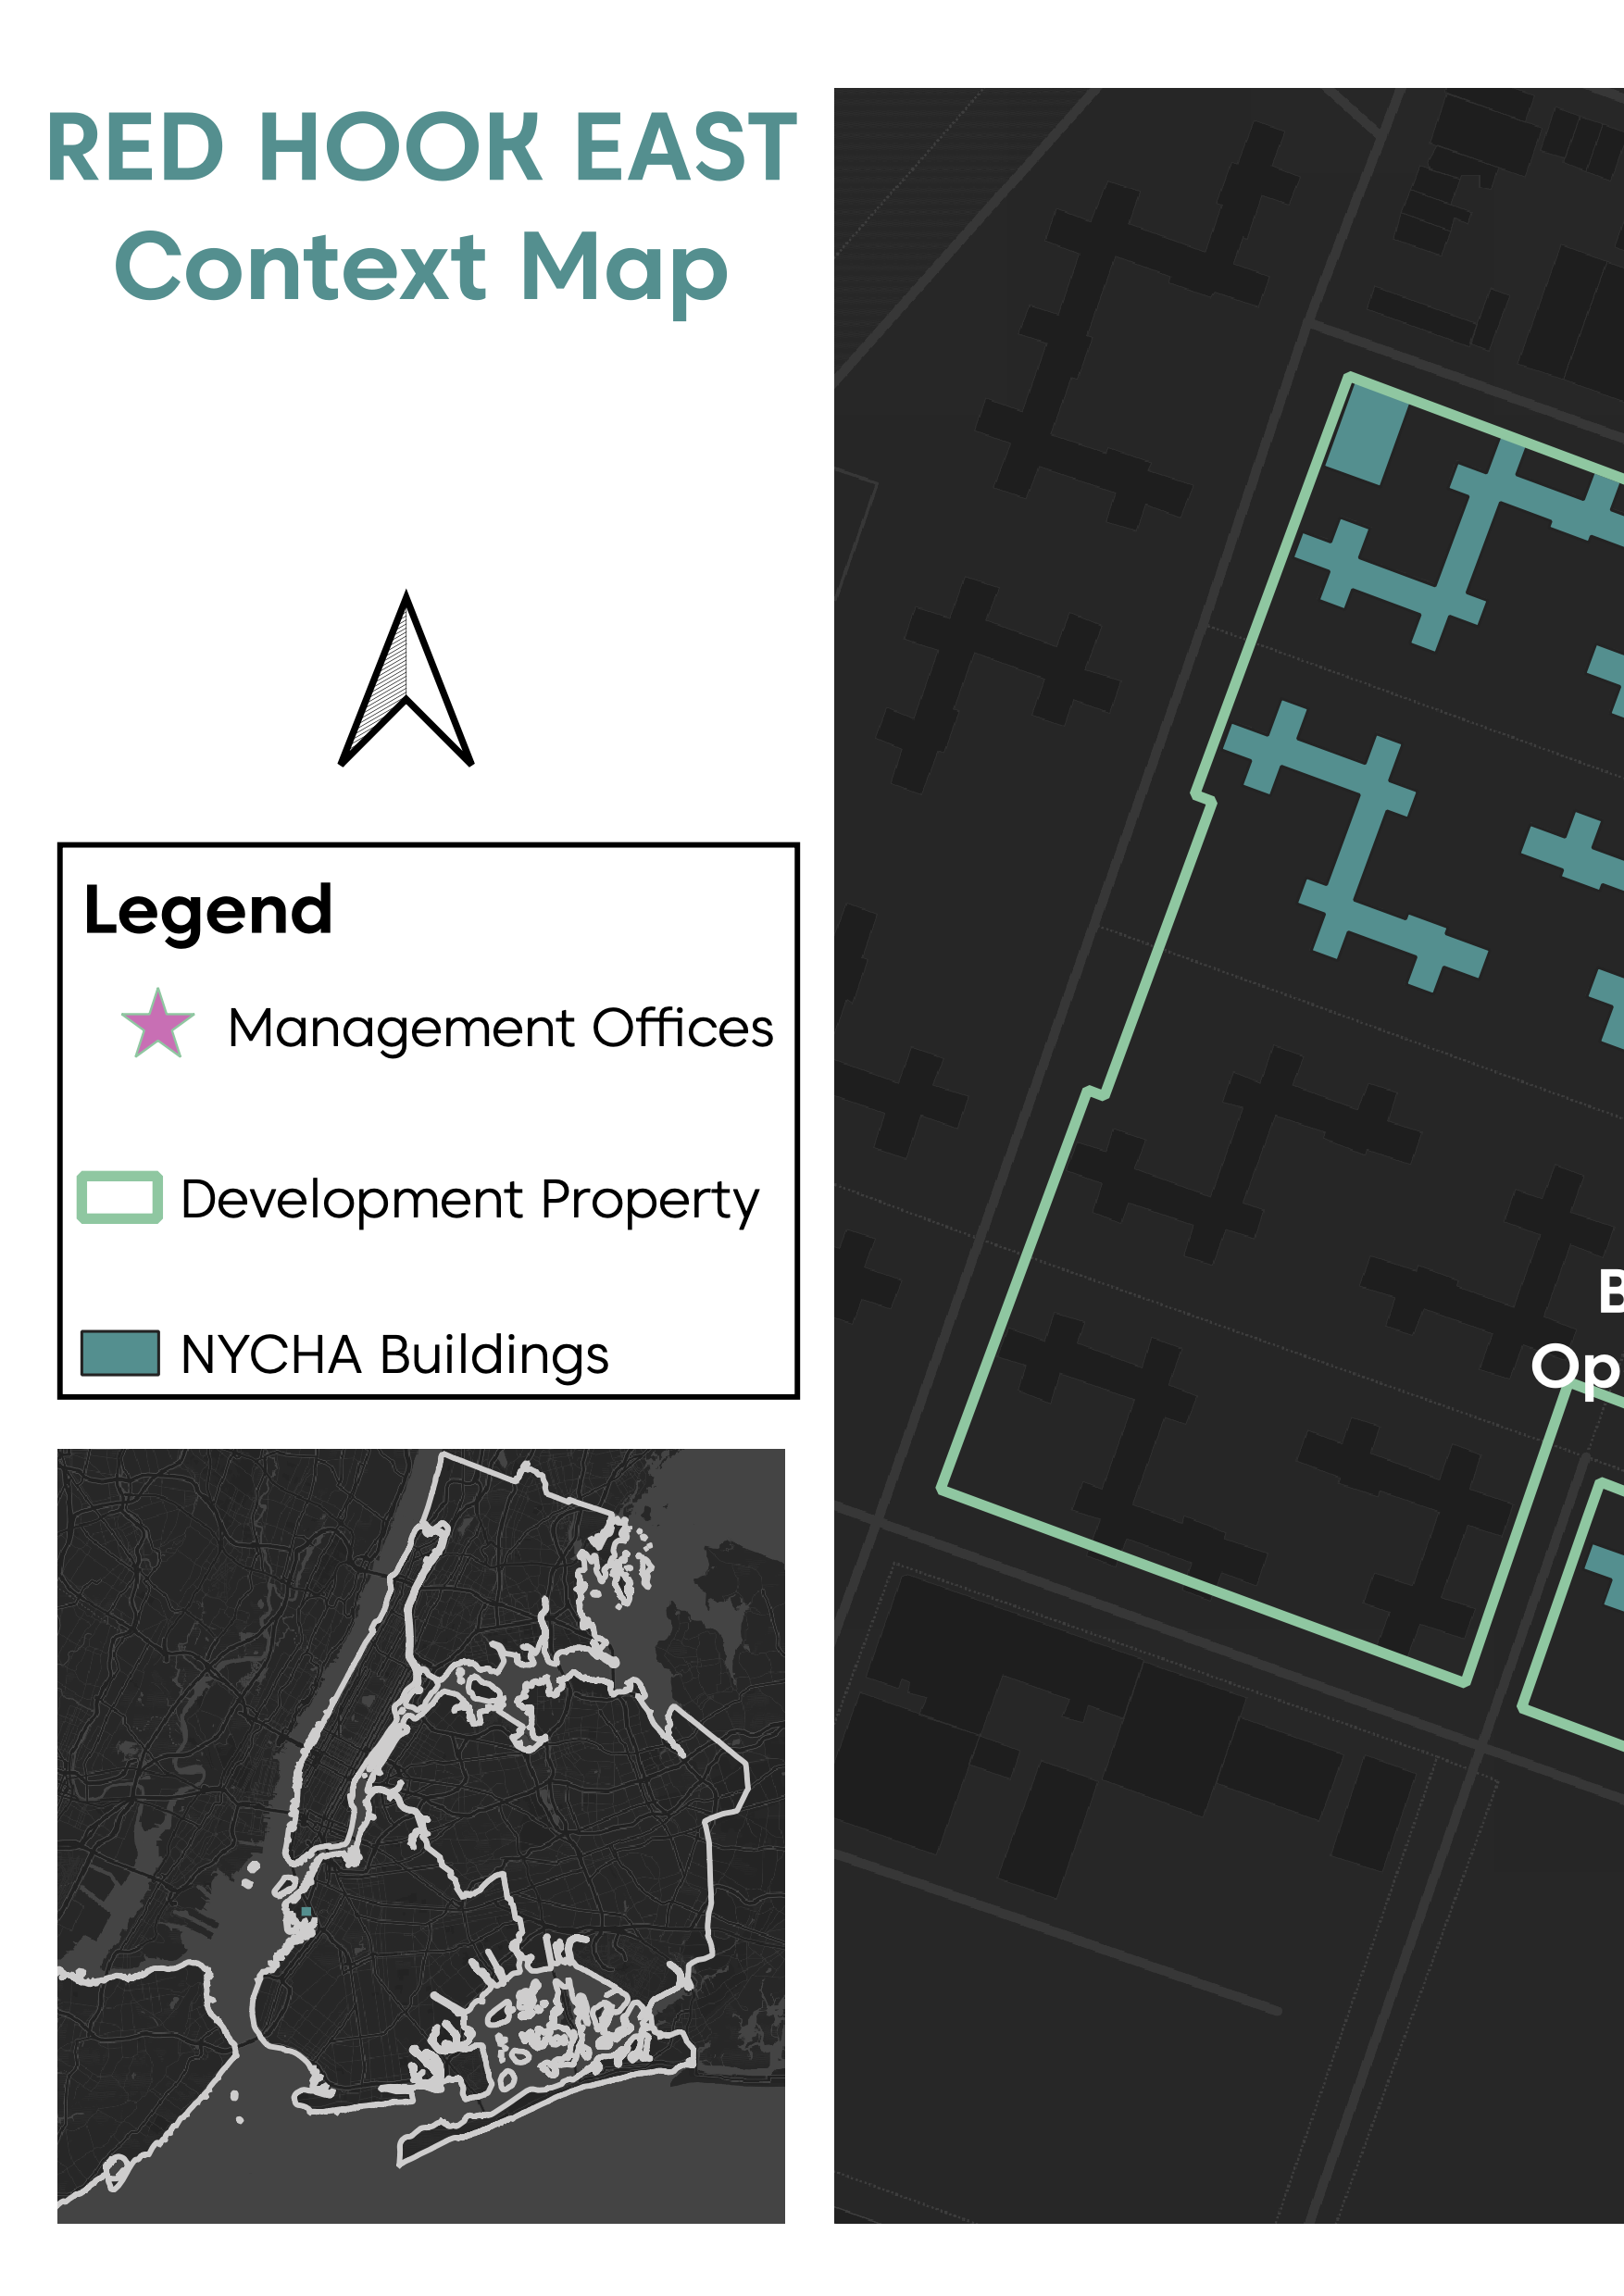
\includegraphics[height=11in]{004_1.png}%
    \end{figure}
    \clearpage
    \begin{figure}[H]
    	\raggedright
        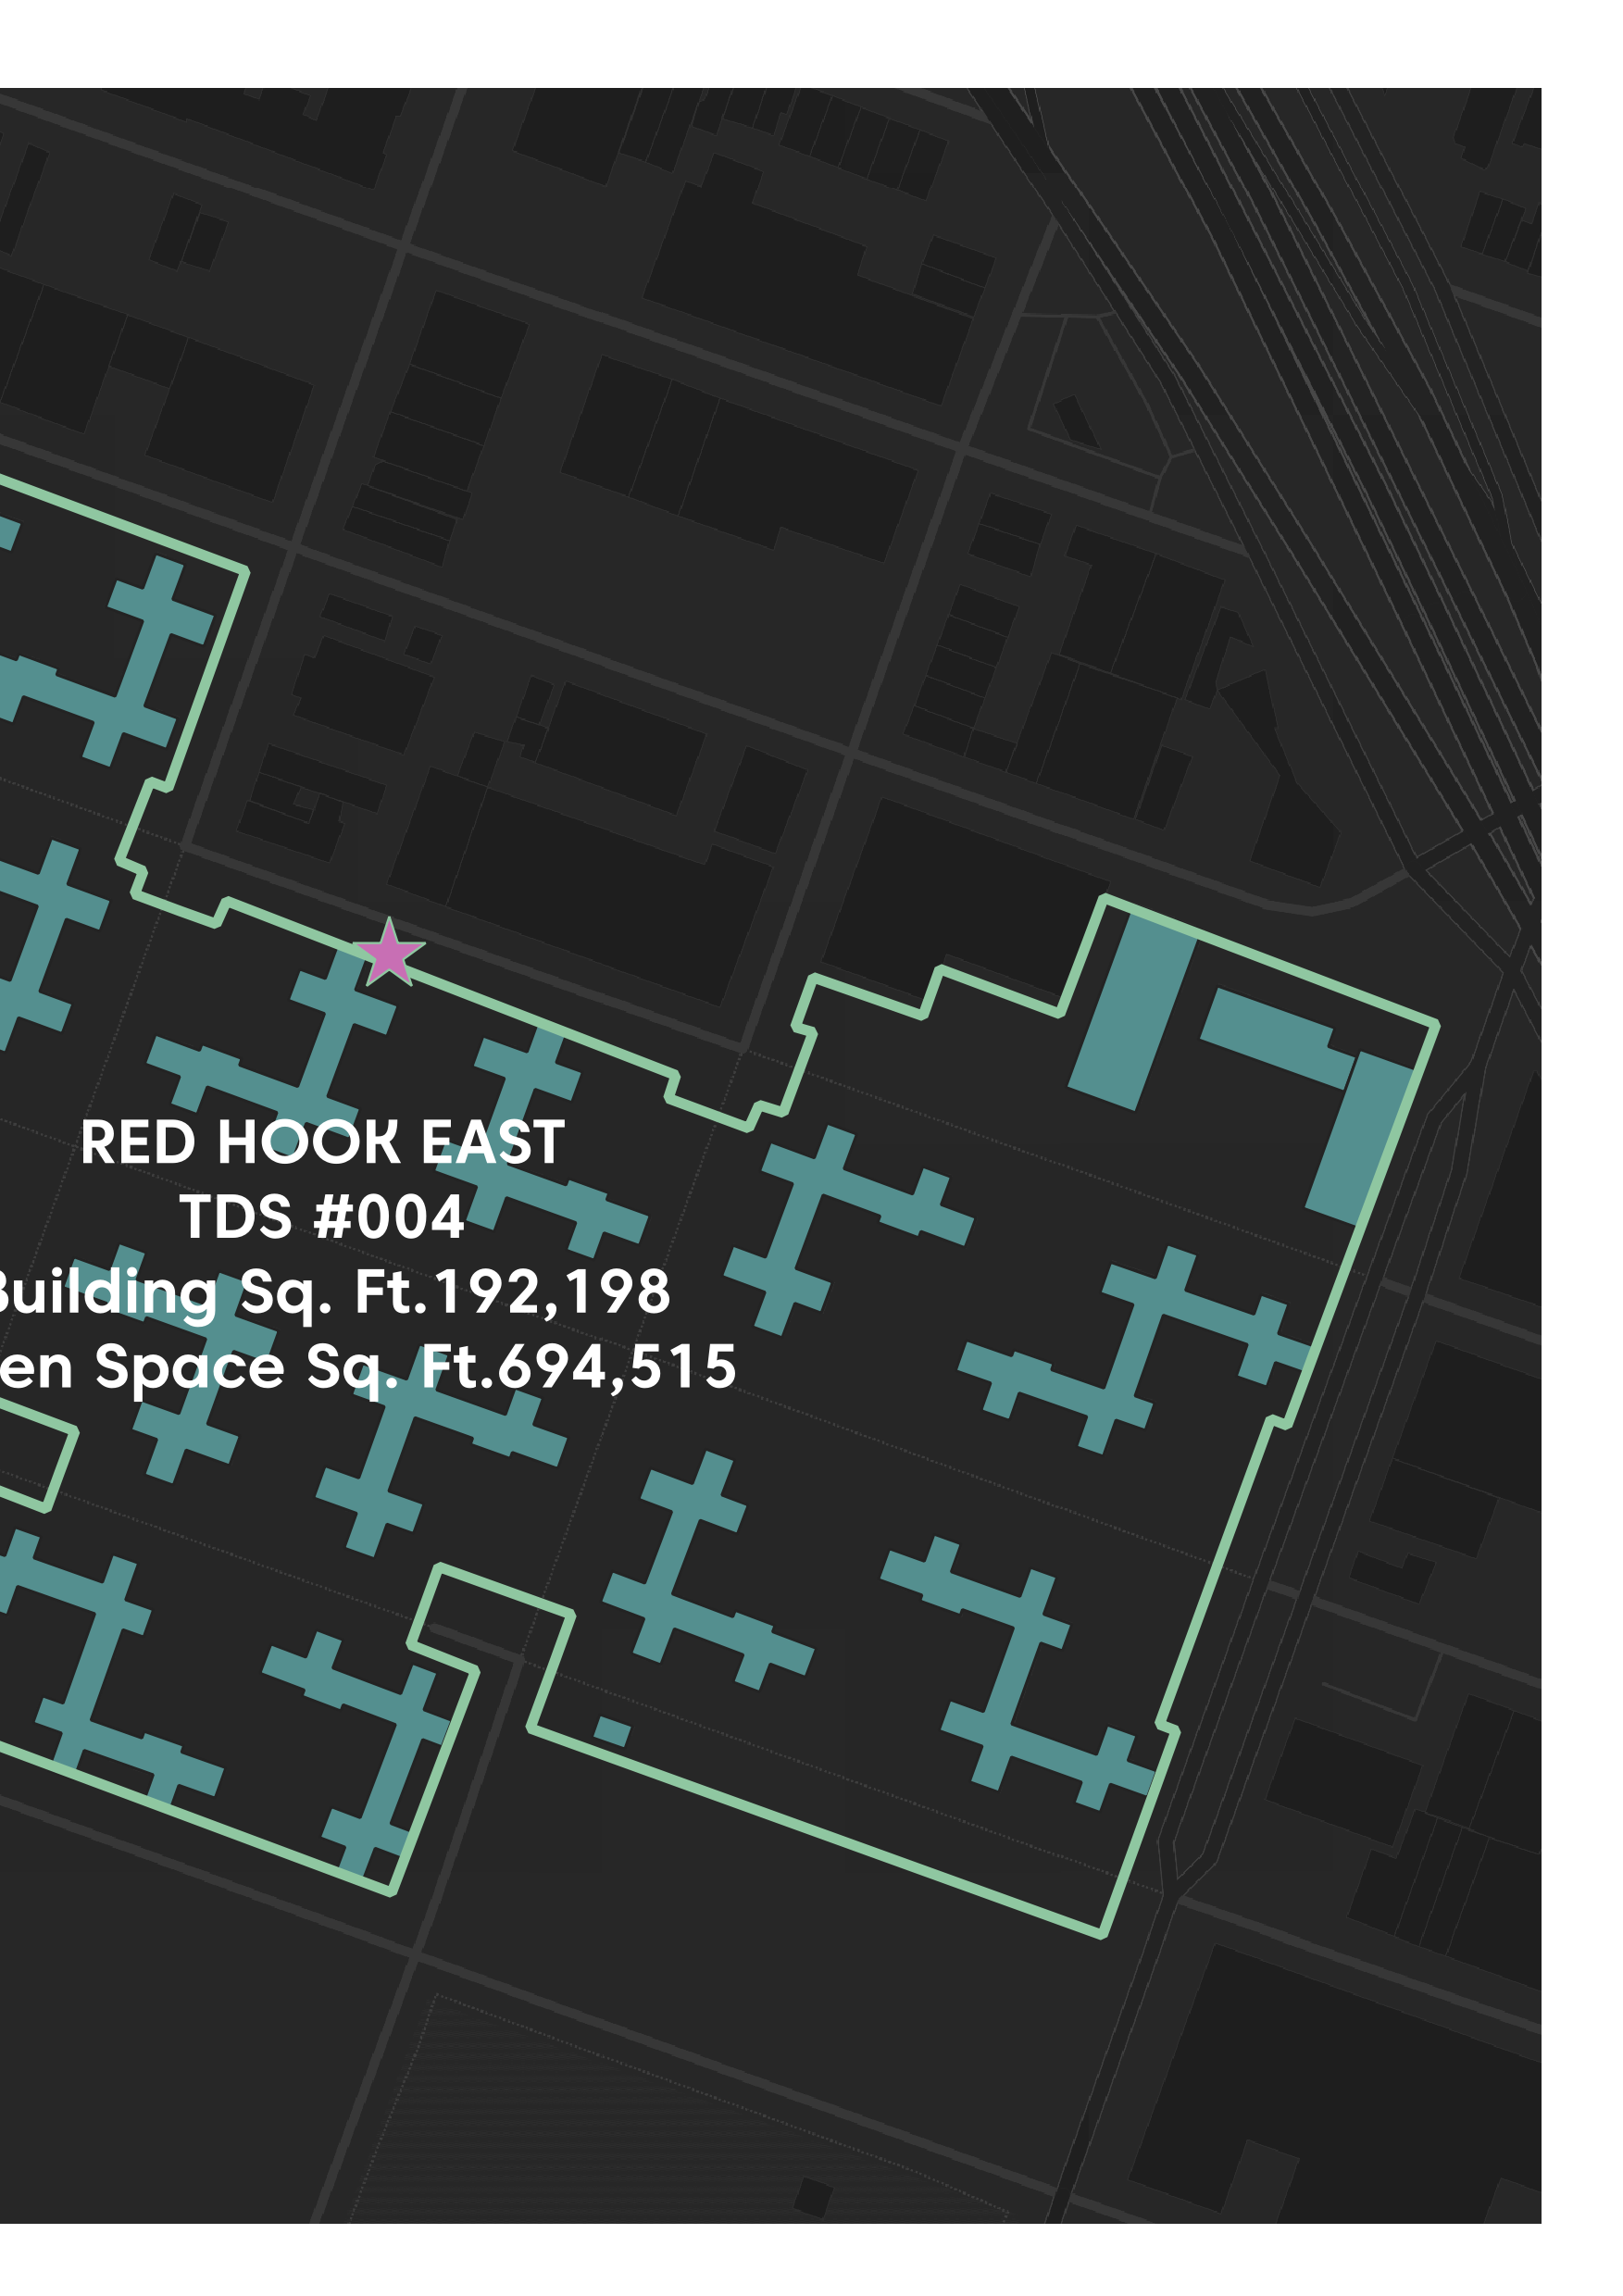
\includegraphics[height=11in]{004_2.png}%
    \end{figure}
    \clearpage
    }%
}
\restoregeometry
\pagebreak
%-------------------------------------------
\pagestyle{plain}
\whitetext{\chapter{Waste Services and Assets}}
\pagecolor{ccorange}
\pagebreak
\newpagecolor{white}
\pagestyle{fancy}
\fancyhf{}
\renewcommand{\chaptermark}[1]{\markboth{#1}{}}
\fancyfoot[LE,RO]{\thepage}

\textcolor{ccorange}{\section{Waste Distribution}}

The goal of the waste calculator is to understand the amount of waste generated at each development and consolidation. This knowledge is imperative to interpreting what assets are necessary in order for each consolidation to run most efficiently. Sumner consolidation is not serviced by DSNY daily. Once the compactors are full, DSNY is called to pick it up. The Sumner Consolidation has (4) 30-CY external compactors and containers, totaling 766.36 ft2 of storage space for waste. Given the rate at which waste is produced at NYCHA properties, these containers will fill up in about (3) days at the Sumner Consolidation. The average weight of the containers at capacity should be about (3) tons.

\begin{table}[H]
\begin{threeparttable}
\small

\textbf{Projected Daily Trash Volumes}
        \begin{tabularx}{\textwidth}{V{1.25in}|X|X|X|X|}
        \cline{2-5}
        
                                                                       & \multicolumn{1}{V{1.25in}|}{\cellcolor{ccorange}{\color[HTML]{FFFFFF}303 Vernon Avenue}}& \multicolumn{1}{V{1.25in}|}{\cellcolor{ccorange}{\color[HTML]{FFFFFF}Bedford-Stuyvesant Rehab}}& \multicolumn{1}{V{1.25in}|}{\cellcolor{ccorange}{\color[HTML]{FFFFFF}Sumner}}& \multicolumn{1}{V{1.25in}|}{\cellcolor{ccorange}{\color[HTML]{FFFFFF}Total}}\tnhl
\multicolumn{1}{|V{1.25in}|}{\cellcolor{ccorangelight}Waste Generated / Day (Tons)\tnote{1}}                 & 0.6                                    & 0.2                                    & 2.7                                    & 3.5                                    \tnhl
\multicolumn{1}{|V{1.25in}|}{\cellcolor{ccorangelight}Trash / Day (tons)\tnote{2}}                 & 0.5                                    & 0.2                                    & 2.5                                    & 3.2                                    \tnhl
\multicolumn{1}{|Y{1.25in}|}{\cellcolor{ccorangelight}Trash Chutes\tnote{3}}                 & 12.1 sausage bags      & 4.4 sausage bags      & 57.0 sausage bags      & 73.5 sausage bags      \tnhl
\multicolumn{1}{|Y{1.25in}|}{\cellcolor{ccorangelight}Drop Sites\tnote{4}}                 & 5.4 64-gal. bins      & 1.9 64-gal. bins      & 25.2 64-gal. bins      & 32.6 64-gal. bins      \tnhl
\multicolumn{1}{|V{1.25in}|}{\cellcolor{ccorangelight}Est. Drop Sites \tnote{5}}                 & 5                                    & 7                                    & 7                                    & 19                                    \tnhl
\end{tabularx}\bigskip\textbf{Projected Weekly Recycling Volumes}
        \begin{tabularx}{\textwidth}{V{1.25in}|X|X|X|X|}
        \cline{2-5}
        
                                                                       & \multicolumn{1}{V{1.25in}|}{\cellcolor{ccorange}{\color[HTML]{FFFFFF}303 Vernon Avenue}}& \multicolumn{1}{V{1.25in}|}{\cellcolor{ccorange}{\color[HTML]{FFFFFF}Bedford-Stuyvesant Rehab}}& \multicolumn{1}{V{1.25in}|}{\cellcolor{ccorange}{\color[HTML]{FFFFFF}Sumner}}& \multicolumn{1}{V{1.25in}|}{\cellcolor{ccorange}{\color[HTML]{FFFFFF}Total}}\tnhl
\multicolumn{1}{|V{1.25in}|}{\cellcolor{ccorangelight}Metal, Glass, Plastic Captured / Week (tons) \tnote{6}}                 & 24.2 44-gal. bags                                   & 8.7 44-gal. bags                                   & 113.4 44-gal. bags                                   & 146.3 44-gal. bags                                   \tnhl
\multicolumn{1}{|V{1.25in}|}{\cellcolor{ccorangelight}Cardboard Captured / Week (tons) \tnote{6}}                 & 19.8 bales                                   & 7.1 bales                                   & 92.9 bales                                   & 119.8 bales                                   \tnhl
\multicolumn{1}{|V{1.25in}|}{\cellcolor{ccorangelight}Paper Captured / Week (tons) \tnote{6}}                 & 2.0 44-gal. bags                                   & 0.7 44-gal. bags                                   & 9.6 44-gal. bags                                   & 12.3 44-gal. bags                                   \tnhl
\end{tabularx}

\begin{tablenotes}
\item [1] Assumes 5lbs of waste is produced daily in each unit.
\item [2] Includes miscellaneous garbage as well as uncaptured recyclables, organics, e-waste, and textiles.
\item [3] Primary method of trash collection, via chute. Assumes a 75\% capture rate.
\item [4] Secondary method of trash collection. Assumes a 25\% capture rate
\item [5] Capture rates of recyclables at NYCHA portfolio-wide: 30\% of MGP, 50\% of Cardboard, and 20\% of Paper. 
%\item[5] Organics, e-waste, and textiles have a capture rate of 0\%.
\end{tablenotes}
\end{threeparttable}
\end{table}
\pagebreak

\textcolor{ccorange}{\section{Waste Services and Assets}}
DSNY does not provide curbside collection at this site. Caretakers are responsible for collecting all
waste throughout the consolidation and bringing it to the external compactors. All bulk is left outside the
buildings for collection to the 30-yard bulk container located at 303 Vernon. Household waste produced
in Sumner goes to one of the three waste yards on site. Household waste produced at
Bedford-Stuyvesant Rehab is brought to the curb for pick up by the caretakers using a Ford pick-up
truck and driven to the waste yards at either Sumner or 303 Vernon.
\begin{table}[H]
\small
\begin{tabular}{V{1.5in}|V{1.5in}|V{1.5in}|V{1.5in}|}
\cline{2-4}
                                                                                   & \cellcolor{ccorange}{\color[HTML]{FFFFFF} 303 Vernon Avenue} & \cellcolor{ccorange}{\color[HTML]{FFFFFF} Bedford-Stuyvesant Rehab} & \cellcolor{ccorange}{\color[HTML]{FFFFFF} Sumner Houses} \\ \hline
\multicolumn{1}{|V{1.5in}|}{\cellcolor{ccorangelight}Household Waste (DSNY)}               & 1 Waste Yard; 1 Hydraulic Exterior Compactor                     & Transfer to 303 Vernon or Sumner                                        & 2  Waste Yards with 1 Hydraulic Exterior Compactor Each      \\ \hline
\multicolumn{1}{|V{1.5in}|}{\cellcolor{ccorangelight}Bulk Waste}                           & IESI with One(?) 30-Yard Container                               & Transfer to 303 Vernon                                                  & Transfer to 303 Vernon                                       \\ \hline
\multicolumn{1}{|V{1.5in}|}{\cellcolor{ccorangelight}Recycling: Paper and Cardboard}       & TK                                                               & TK                                                                      & TK                                                           \\ \hline
\multicolumn{1}{|V{1.5in}|}{\cellcolor{ccorangelight}Recycling: Metal, Glass, and Plastic} & DSNY Curb Setout                                                 & DSNY Curb Setout                                                        & DSNY Curb Setout                                             \\ \hline
\multicolumn{1}{|V{1.5in}|}{\cellcolor{ccorangelight}Recycling: Mattresses}                & N/A                                                              & N/A                                                                     & TK                                                           \\ \hline
\multicolumn{1}{|V{1.5in}|}{\cellcolor{ccorangelight}Recycling: Textiles}                  & N/A                                                              & N/A                                                                     & TK                                                           \\ \hline
\multicolumn{1}{|V{1.5in}|}{\cellcolor{ccorangelight}Recycling: E-Waste}                   & N/A                                                              & N/A                                                                     & TK                                                           \\ \hline
\end{tabular}
\end{table}
\pagebreak

\textcolor{ccorange}{WASTE ASSET MAP}
\begin{figure}[H]
\raggedright
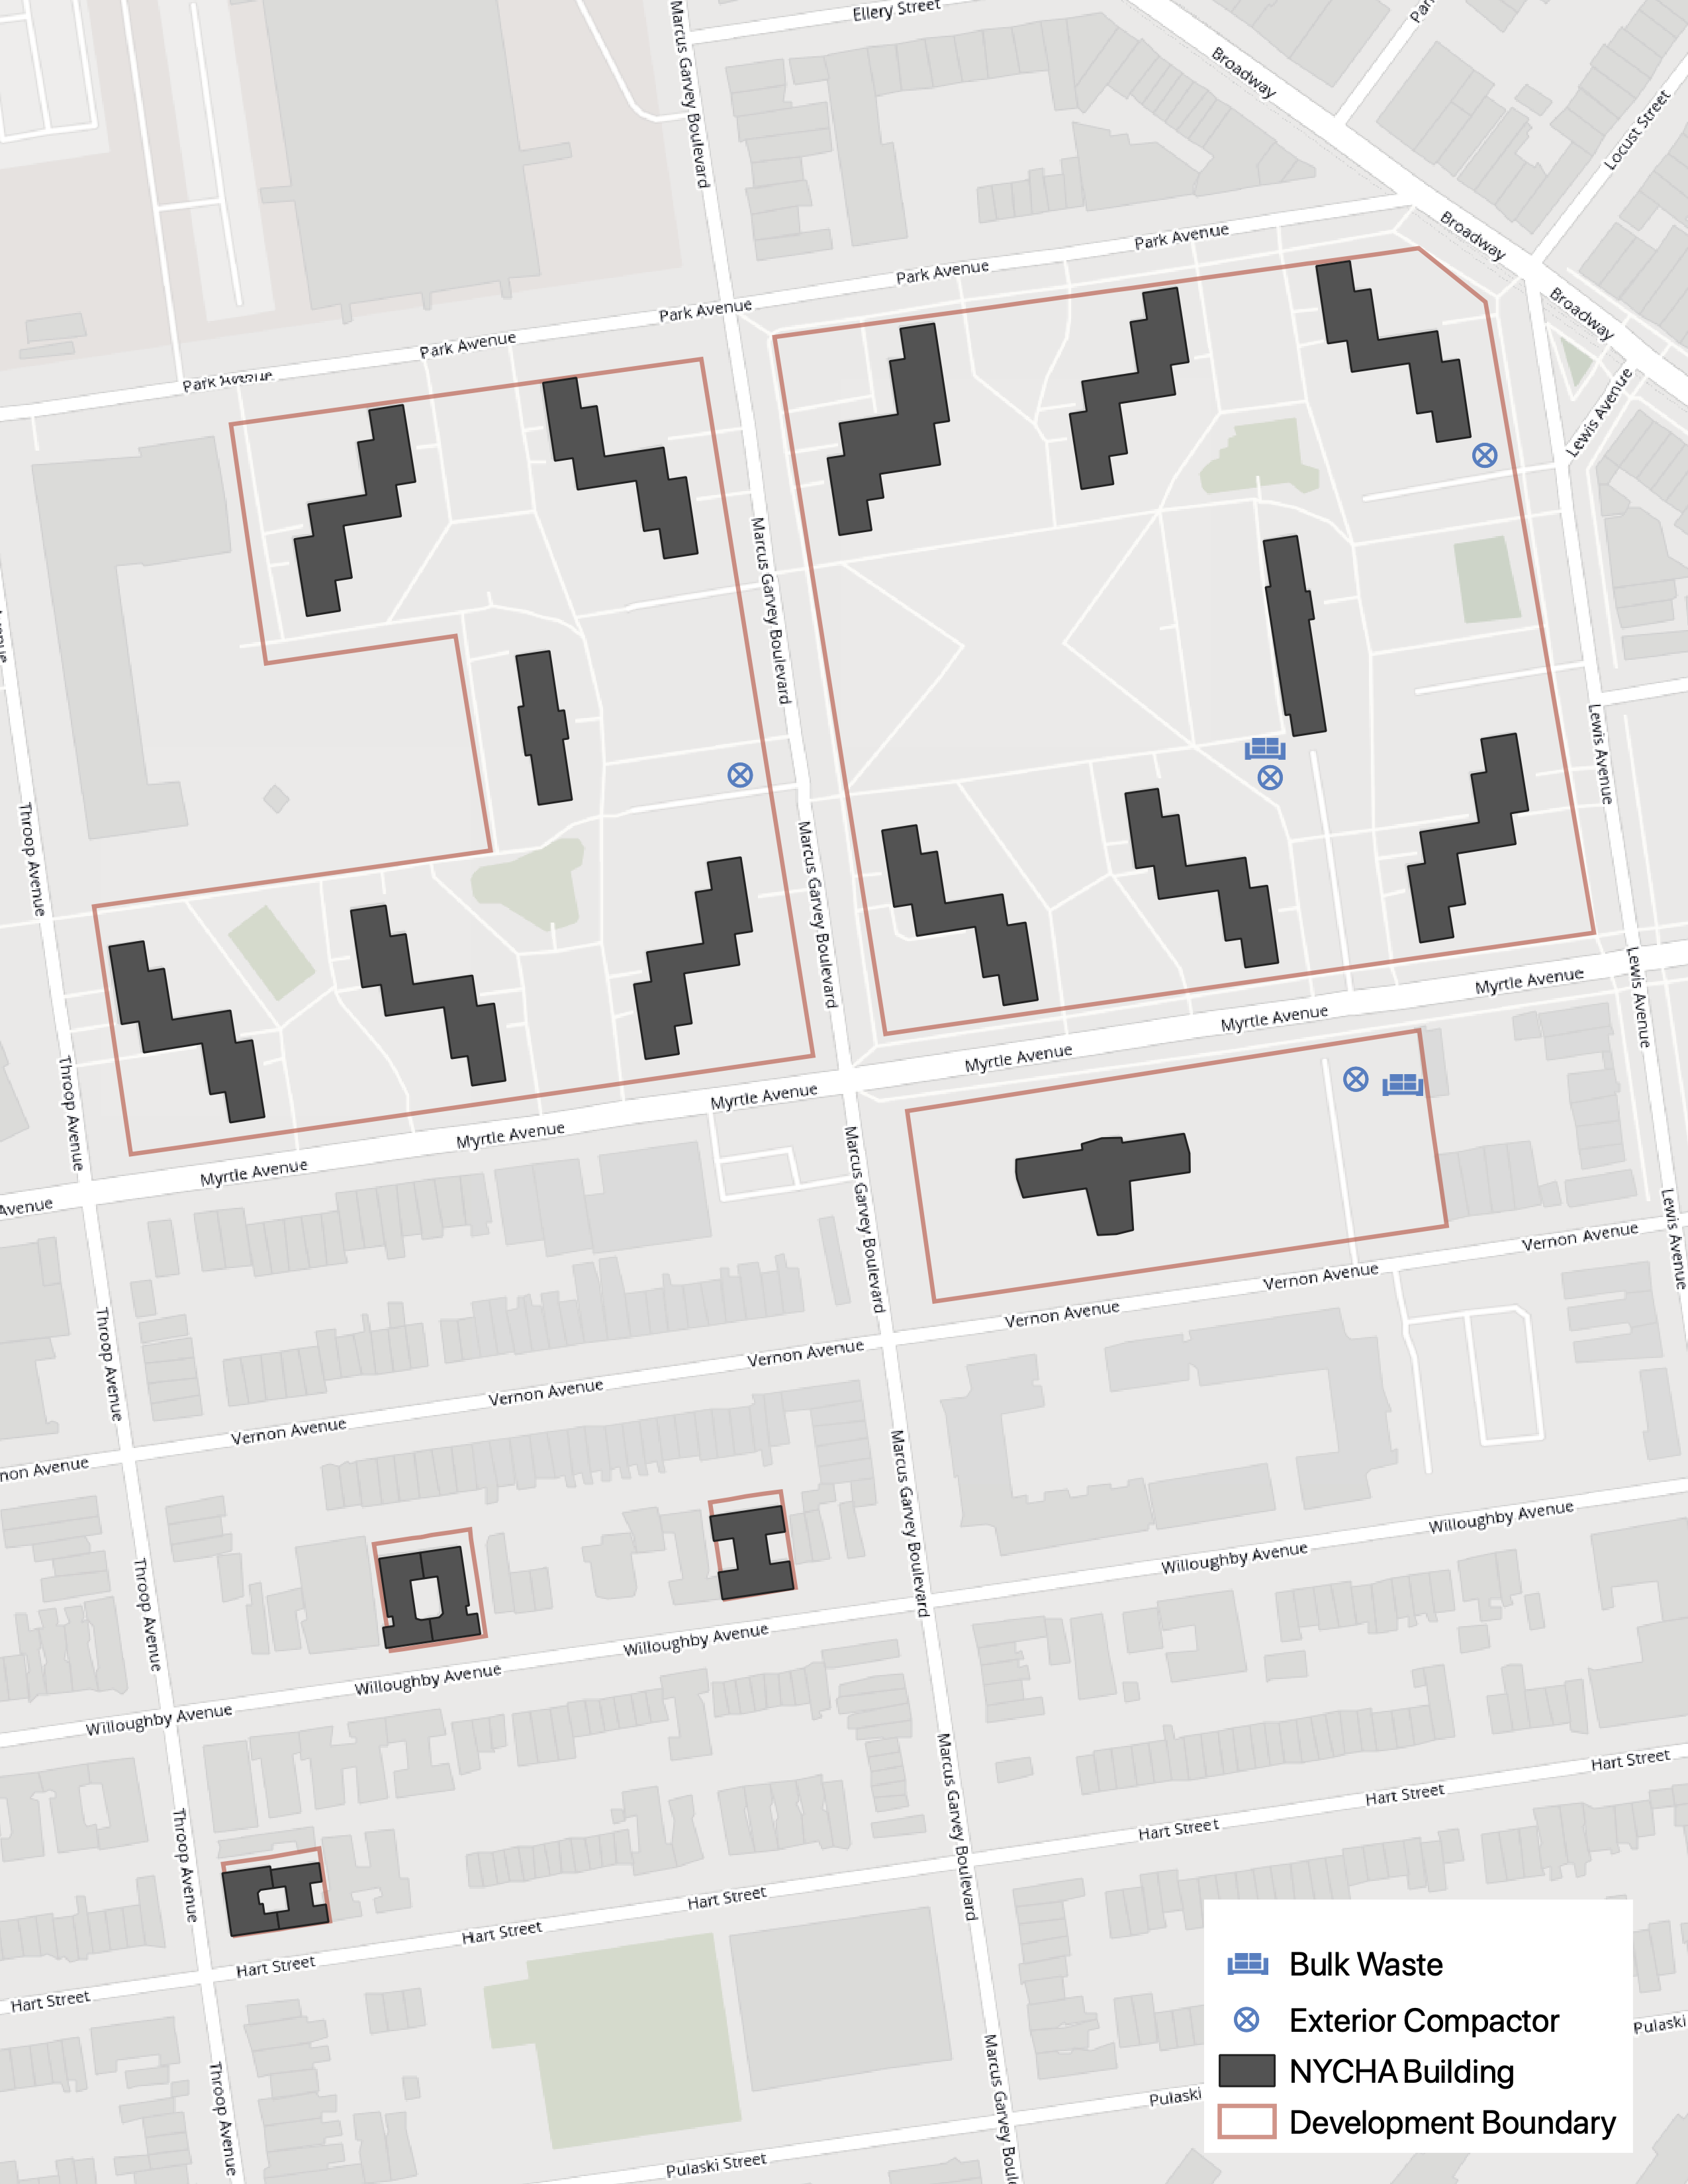
\includegraphics[width=.95\textwidth]{073_asset_map.png}
\end{figure}
\pagebreak

\textcolor{ccorange}{WASTE ASSETS}

\begin{table}[H]
\small
\begin{tabular}{V{.25\columnwidth}|V{.15\columnwidth}|V{.15\columnwidth}|V{.25\columnwidth}|V{.15\columnwidth}|}
\cline{2-5}
                                                                                              & \cellcolor{ccorangelight}{\color[HTML]{000000} Internal Compactors} & \cellcolor{ccorangelight}{\color[HTML]{000000} External Compactors} & \cellcolor{ccorangelight}{\color[HTML]{000000} Other External Assets}   & \cellcolor{ccorangelight}{\color[HTML]{000000} Recycling Bins} \\ \hline
\multicolumn{1}{|V{.25\columnwidth}|}{\cellcolor{ccorange}{\color[HTML]{FFFFFF} 303 Vernon Avenue}}        & 1; last replaced TK                                                & 1                                                                  & Bulk crusher, cardboard baler, mattress recycling, electric tilt truck & TK                                                            \\ \hline
\multicolumn{1}{|V{.25\columnwidth}|}{\cellcolor{ccorange}{\color[HTML]{FFFFFF} Bedford-Stuyvesant Rehab}} & 5; last replaced TK                                                & 0                                                                  & Bulk crusher, cardboard baler, mattress recycling, electric tilt truck & TK                                                            \\ \hline
\multicolumn{1}{|V{.25\columnwidth}|}{\cellcolor{ccorange}{\color[HTML]{FFFFFF} Sumner Houses}}            & 24; last replaced TK                                               & 3                                                                  & Bulk crusher, cardboard baler, mattress recycling, electric tilt truck & TK                                                            \\ \hline
\end{tabular}
\end{table}

\textcolor{ccorange}{SUMNER CONSOLIDATION ASSETS}
\begin{table}[H]
\begin{tabular}{m{.33\columnwidth}m{.33\columnwidth}m{.33\columnwidth}}
{\color{ccorange} X Trucks} & {\color{ccorange} X Bobcats} & {\color{ccorange} X Other} \\

\includegraphics[width=.25\columnwidth]{truck.png}                            & 
\includegraphics[width=.25\columnwidth]{bobcat.png}                             & 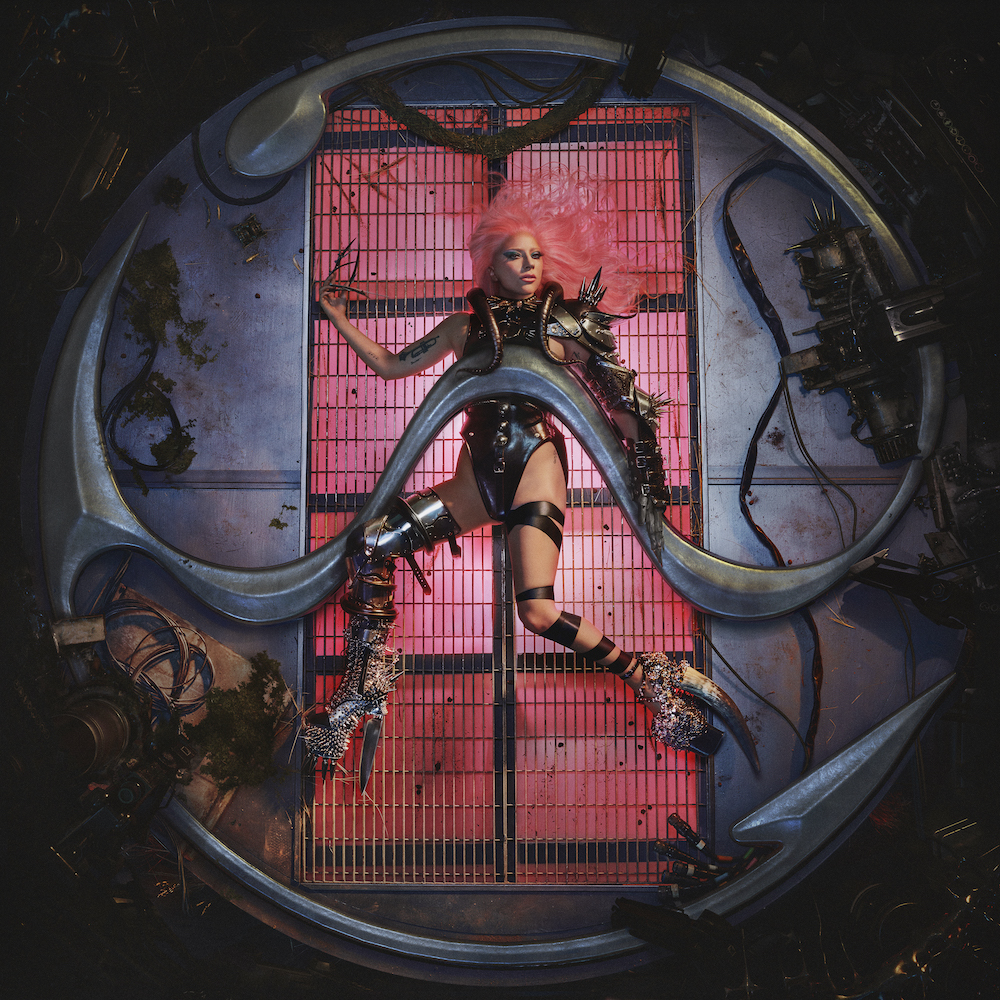
\includegraphics[width=.25\columnwidth]{chromatica.jpg}                          
\end{tabular}
\end{table}
\pagebreak
\textcolor{ccorange}{\section{Capital Improvements}}

\begin{table}[H]


\begin{tabularx}{\textwidth}{r|X|X|X|}
\cline{2-3}
\multicolumn{1}{l|}{}                                                        & \cellcolor{ccorange}{\color[HTML]{FFFFFF}303 Vernon Avenue} & \cellcolor{ccorange}{\color[HTML]{FFFFFF}Bedford-Stuyvesant Rehab} & \cellcolor{ccorange}{\color[HTML]{FFFFFF}Sumner} \\ \hline
\multicolumn{1}{|V{.2\columnwidth}|}{\cellcolor{ccorangelight}In-Sink Food Grinders}          &                                                                  &                                                                  &                                                                  \\
\multicolumn{1}{|r|}{\cellcolor{ccorangelight}\textit{Status}}                & Estimate                                                         & Estimate                                                         & Estimate                                                         \\
\multicolumn{1}{|r|}{\cellcolor{ccorangelight}\textit{Cost}}                  & \$402,184.21  (est.)                                                     & \$144,373.82  (est.)                                                     & \$1,887,172.07  (est.)                                                     \\ \hline
\multicolumn{1}{|V{.2\columnwidth}|}{\cellcolor{ccorangelight}Enlarged Hopper Doors}          &                                                                  &                                                                  &                                                                  \\
\multicolumn{1}{|r|}{\cellcolor{ccorangelight}\textit{Status}}                & Queued                                                         & Queued                                                         & Completed                                                         \\
\multicolumn{1}{|r|}{\cellcolor{ccorangelight}\textit{Cost}}                  & \$7,435.64  (est.)                                                     & \$37,178.22  (est.)                                                     & \$148,620.14                                                      \\ \hline
\multicolumn{1}{|V{.2\columnwidth}|}{\cellcolor{ccorangelight}Interior Compactor Replacement}          &                                                                  &                                                                  &                                                                  \\
\multicolumn{1}{|r|}{\cellcolor{ccorangelight}\textit{Status}}                & Queued                                                         & In Progress                                                         & Completed                                                         \\
\multicolumn{1}{|r|}{\cellcolor{ccorangelight}\textit{Cost}}                  & \$63,087.50  (est.)                                                     & \$247,785.00 (est.)                                                     & \$957,660.00  (est.)                                                     \\ \hline
\multicolumn{1}{|V{.2\columnwidth}|}{\cellcolor{ccorangelight}Waste Yard Redesign}          &                                                                  &                                                                  &                                                                  \\
\multicolumn{1}{|r|}{\cellcolor{ccorangelight}\textit{Status}}                & Estimate                                                         & Estimate                                                         & Estimate                                                         \\
\multicolumn{1}{|r|}{\cellcolor{ccorangelight}\textit{Cost}}                  & \$1,870,809.86  (est.)                                                     & \$1,934,073.96  (est.)                                                     & \$1,552,980.79  (est.)                                                     \\ \hline
\end{tabularx}

\end{table}
\pagebreak

\textcolor{ccorange}{PRIORITIES}

PLACEHOLDER TEXT AND TABLES AND SUCH TO FIGURE OUT PAGE COLOR SETTINGS -- WILL FILL IN LATER, ONCE PRELIMINARY ANALYSIS IS COMPLETE
\pagebreak
%-------------------------------------------
\pagestyle{plain}
\whitetext{\Chapter{Staffing}}
\pagecolor{ccfuschia}
\pagebreak
\newpagecolor{white}
\pagestyle{fancy}
\fancyhf{}
\renewcommand{\chaptermark}[1]{\markboth{#1}{}}
\fancyfoot[LE,RO]{\thepage}


\textcolor{ccfuschia}{STAFFING STRUCTURE}
\begin{figure}[H]
	\resizebox{\textwidth}{!}{
	\centering
	\begin{tikzpicture}[node distance=3cm]
	\node (vp) [processwide] {VP of Operations};
	\node (borodr) [processwide, below of=vp] {Borough Director};
	\node(ram) [processwide, below of=borodr] {Regional Asset Manager};
	\node (pm) [processwide, below of=ram] {Property Manager};
	\node (super) [process, below of=pm, xshift=-5cm] {Superintendent};
	\node (asuper) [process, below of=super] {Assistant Superintendent};
		\node (mtn) [process, below of=asuper, xshift=-3.5cm] {Maintenance Workers};
		\node (spc) [process, below of=asuper] {Supervisor of Caretakers};
			\node (crt) [process, below of=spc] {Caretakers\\(X and J)};
		\node (spg) [process, below of=asuper, xshift=3.5cm] {Supervisor of Grounds};
			\node (crtg) [process, below of = spg] {Caretakers (G)};			
		
	\node (apm)[process, below of=pm, xshift=5cm] {Assistant Property Manager};
		\node (sec) [process, below of=apm, xshift = -2.5cm] {Secretaries};
		\node (asst) [process, below of=apm, xshift = 2.5cm] {Housing Assistants};

	%\node (sub1) [subprocess, below of=pro1] {\nodepart{two} Subprogram};
	%\node (dec1) [decision, below of=sub1, yshift=-1cm] {Decision};
	%\node (com1) [comment, below of=dec1, xshift=-4cm, yshift=-1cm] {STEP 2};
	%\node (stop) [startstop, below of=dec1, yshift=-1cm] {Stop};

	%\draw [arrow] (dec1.west) -- ++(-1,0) node[anchor=south,pos=0.5] {No} |- (sub1.west);
	%\draw [arrow] (dec1) -- node[anchor=west] {Yes} (stop);

	\draw [arrow] (vp) -- (borodr);
	\draw [arrow] (borodr) -- (ram);
	\draw [arrow] (ram) -- (pm);
	\draw [arrow] (pm) -- (super);
	\draw [arrow] (super) -- (asuper);
		\draw [arrow] (asuper) -- (mtn);
		\draw [arrow] (asuper) -- (spc);
			\draw [arrow] (spc) -- (crt);
		\draw [arrow] (asuper) -- (spg);
			\draw [arrow] (spg) -- (crtg);
	
	\draw [arrow] (pm) -- (apm);
		\draw [arrow] (apm) -- (sec);
		\draw [arrow] (apm) -- (asst);
	\end{tikzpicture}
	}
\end{figure}

\pagebreak
\textcolor{ccfuschia}{ALLOCATED STAFF}

\begin{table}[H]
\begin{threeparttable}


        \begin{tabular}{l|c|c|c|}
        \cline{2-4}
                                                                                     & \cellcolor{ccfuschia}{\color[HTML]{FFFFFF} Formula Allocation} & \cellcolor{ccfuschia}{\color[HTML]{FFFFFF} Budgeted} & \cellcolor{ccfuschia}{\color[HTML]{FFFFFF} Actual} \\ \hline
        \multicolumn{1}{|l|}{\cellcolor{ccfuschialight}Employees}                      & 45                                                      & 46                                                                & 41                                                        \\ \hline
        \multicolumn{1}{|l|}{\cellcolor{ccfuschialight}Property Manager}               & 1                                                      & 1                                                                & 1                                                       \\ \hline
        \multicolumn{1}{|l|}{\cellcolor{ccfuschialight}Asst. Property Manager}         & 1                                                      & 1                                                                & 1                                                       \\ \hline
        \multicolumn{1}{|l|}{\cellcolor{ccfuschialight}Secretaries}                    & 2                                                      & 2                                                                & 2                                                      \\ \hline
        \multicolumn{1}{|l|}{\cellcolor{ccfuschialight}Housing Assistants}             & 4                                                      & 4                                                                & 4                                                      \\ \hline
        \multicolumn{1}{|l|}{\cellcolor{ccfuschialight}Superintendent}                 & 1                                                      & 1                                                                & 1                                                      \\ \hline
        \multicolumn{1}{|l|}{\cellcolor{ccfuschialight}Assistant Superintendent}       & 2                                                      & 2                                                                & 2                                                      \\ \hline
        \multicolumn{1}{|l|}{\cellcolor{ccfuschialight}Supervisor of Caretakers (SOC)} & 1                                                      & 1                                                                & 1                                                      \\ \hline
        \multicolumn{1}{|l|}{\cellcolor{ccfuschialight}Supervisor of Grounds (SOG)}    & 1                                                      & 1                                                                & 1                                                      \\ \hline
        \multicolumn{1}{|l|}{\cellcolor{ccfuschialight}Maintenance Workers}            & 6                                                      & 6                                                                & 3                                                       \\ \hline
        \multicolumn{1}{|l|}{\cellcolor{ccfuschialight}Caretakers X}                   & 5                                                      & 5                                                                &                                                       \\ \cline{1-3}
        \multicolumn{1}{|l|}{\cellcolor{ccfuschialight}Caretakers J\tnote{1}}                   &                                                       & 20                                                                &                                                         \\ \cline{1-1} \cline{3-3}
        \multicolumn{1}{|l|}{\cellcolor{ccfuschialight}Caretakers G}                   & \multirow{-2}{*}{21}                                                      & 2                                     & \multirow{-3}{*}{25}                           \\ \hline
        \end{tabular}
        
        

\begin{tablenotes}
\item [1] Includes staff in roles Caretaker J, Caretaker I, and Chief Caretaker
\end{tablenotes}
\end{threeparttable}
\end{table}

\pagebreak
%-------------------------------------------
\pagestyle{plain}
\whitetext{\Chapter{Analysis}}
\pagecolor{ccgreen}
\pagebreak
\newpagecolor{white}
\pagestyle{fancy}
\fancyhf{}
\renewcommand{\chaptermark}[1]{\markboth{#1}{}}
\fancyfoot[LE,RO]{\thepage}
\textcolor{ccgreen}{ANALYSIS OF FINDINGS}
\\
\emph{Inspection and Collection Requirement}

Sumner Consolidation is in compliance with the inspection and collection requirement of  Paragraph 45 of the HUD Agreement, according to a Compliance Interview conducted on November 21, 2019. The Supervisor of Grounds, Dirk Jacob, reported they have sufficient manpower to correct all observed deficiencies. NYCHA caretakers conduct ground inspections, picked up litter from the grounds and removed trash from the buildings one to two times a day including weekends. The caretakers begin picking up trash out each day between 8:00 AM -- 10:00 AM and stop between 4:00 PM -- 5:00 PM.  

\emph{Removal and Storage Requirement}

Sumner Consolidation is in compliance with the storage and removal of Paragraph 45 of the HUD Agreement. Despite trash only being removed 2 times a week by DSNY, on days where waste is not removed, Sumner Consolidation can store waste in a manner that prevents access by pests and is thus in compliance.  

DSNY comes Tuesdays and Fridays and Saturdays. Due to the infrequency of DSNY, waste is not removed from the premises daily. An average of five to six bulk tickets are created each week for the removal of bulk waste. Bulk trash sits in a yard with an exterior container before being picked up by the vendor. 

In terms of storage, in addition to depositing litter into interior trash chutes, residents of this consolidation may drop their waste at 13 additional sites on the premises. Tenants are asked by management to leave their trash in the front of each building, either in trash cans or in exposed trash bags for pick up by caretakers if they choose not to use the chutes. Most tenants dispose of their trash using these drop-off sites. Waste is taken to one of four exterior compactors after being taken from the drop-off sites. All exterior compactors are in good shape and do not require maintenance at the time of reporting. When the trash is not removed from the premises, it is stored in a way that prevents pests. 

Sumner has two bulk containers and 31 interior compactor rooms. Of the 31 interior compactor rooms, two were inaccessible due to pests (67 Marcus Garvey Boulevard) and one due to flooding (987 Myrtle Avenue). Sumner disposes of approximately 100 -- 200 compactor bags. The supervisor also stated that Sumner did not have a pest problem and treated any pest problems by collapsing the burrows. According to the Rat Reduction Plan, in the summer of 2018, the site had 61 rat burrows, but as of March 13, 2019, they have very few burrows. Further research is needed to quantify the number of borrows still. 

Sumner reports that, if necessary, they can take the trash from the developments to Tompkins Houses, Marcy Houses, and Roosevelt Houses and vice versa. According to the compliance report, there are external sources of waste and bulk being illegally dumped at this site, primarily from construction companies, stores, and unknown sources. According to Mr. Jacob, the biggest obstacle the site faces is insufficient staffing and that resident outreach was the primary way to improve trash management.  

In a June 24, 2020 report, the Monitor Cleanliness Team gave 303 Vernon a B- and Sumner an overall B grade. The team has not yet evaluated Bedford-Stuyvesant Rehab.  

\pagebreak
% ############################################
\pagestyle{plain}
\whitetext{\Chapter{Appendices}}
\pagecolor{lightBlue}
\pagebreak
\newpagecolor{white}
\pagestyle{fancy}
\fancyhf{}
\renewcommand{\chaptermark}[1]{\markboth{#1}{}}
\fancyfoot[LE,RO]{\thepage}
\textcolor{darkBlue}{Appendix I}

PLACEHOLDER

\pagebreak

% ############################################

% ############################################
\begin{comment}

\section{Lists}

Unordered Lists:
\begin{itemize}
\item This is an unordered list. 
\item Item 2.
\item It has three items.
\end{itemize}

Ordered List:
\begin{enumerate}
\item This is an ordered list.
\item Item 2.
\item It has three items.
\end{enumerate}

Ordered List (alphabetical):
\begin{enumerate}[label=\Alph*.]
\item This is an ordered list.
\item Item 2.
\item It has three items.
\end{enumerate}

% ----------------------------------------------
\cleardoublepage
\chapter{Figures}\label{ch:figures}

% ############################################
\section{Images}\label{sec:images}

\autoref{fig:image1} shows how to display images.

\begin{figure}[H]
	\centering
	\includegraphics[width=0.5\textwidth]{example-image-a.pdf}
	\caption{Image}

	\label{fig:image1}
\end{figure}

\begin{figure}[H]
	\centering
	\includegraphics[width=0.5\textwidth]{example-image-b.pdf}
	\caption{Image with Source}
	\captionsource{\cite{mus:16}}	
	\label{fig:image2}
\end{figure}

\begin{figure}[H]
	\centering
	\includegraphics[width=0.5\textwidth]{example-image-c.pdf}
	\caption{Image with Source and Link}
	\captionsource[https://example.org]{J. Doe}	
	\label{fig:image3}
\end{figure}

% ############################################

% ----------------------------------------------
\cleardoublepage
\chapter{Conclusion}\label{ch:conclusion}

\end{comment}

